\section{Evaluation of community detection
methods}\label{evaluation-of-community-detection-methods}

The lack of consensus on exactly what a community is and what is meant
to be achieved by its detection has presented problems for the
evaluation of community detection methods. Still, attempts have been
made to systematically evaluate the performance and output of different
methods.

Evaluating the results of any community detection method can be thought
in terms of either \emph{internal} or \emph{external} validity. Measures
of \emph{internal} validity evaluate the output of a clustering
algorithm according to some quality measure that uses only the
properties of this output; these include modularity
\autocite{newman_finding_2004}, minimum description length
\autocite{rosvall_map_2010}, and conductance
\autocite{leskovec_empirical_2010}. These measures are designed to
measure how well the communities identified by a method adhere to some
mathematical definition of what a proper community structure should look
like. The problem with using these measures to evaluate and compare
methods is that these measures often serve as the objective functions
for the very algorithms we want to evaluate. While it may be useful to
use these quality measures to compare algorithms that are trying to
optimize the same function, it may not be fair to compare more broadly
than this. As there is no strict mathematical definition for a
community, different algorithms use different quality functions to
surface community structure, and those algorithms that optimize for
whatever measure we are using to evaluate would have an unfair
advantage. Some of these quality measures are discussed in the previous
section on existing community detection algorithms.

Because of this, much of the work around evaluating community detection
methods has focused on \emph{external} validity measures, in which the
input is a network with a known community structure. The evaluation in
this case measures how well the community detection method matches this
ground truth. These ``gold standard'' networks used for evaluation are
either (1) synthetic benchmark networks created with planted
communities, or (2) real-world networks with known metadata which are
treated as ground-truth communities. In either case, the results of a
community detection algorithm can be evaluated against the expected
structure using some comparison measure.

\hypertarget{comparison-measures}{\subsection{Comparison
measures}\label{comparison-measures}}

Evaluating a community detection method against either a synthetic
benchmark network or a real-world network with known community structure
requires some measure of comparison between the clustering found by the
method and the ground truth clustering. The popular measures that have
been adopted fall into one of three categories: (1) measures based on
\emph{pair counting}, (2) measures based on \emph{set matching}, or (3)
measures based on \emph{information theory}
\autocites{meila_comparing_2007}{vinh_information_2010}. These are all
general measures comparing data (not just network) clusterings; they
work by viewing the network as data points with communities as cluster
assignments.

\emph{Pair counting measures} work by taking every possible pair of
nodes in the network and classifying them based on their co-occurrence
in the clusterings. Each of these categories is then counted:

\begin{itemize}
\tightlist
\item
  \(N_{11}\): the number of pairs that co-occur in the same cluster in
  both clusterings
\item
  \(N_{00}\): the number of pairs that do not co-occur in either
  clustering
\item
  \(N_{10}\) or \(N_{01}\): the number of pairs that co-occur in one
  clustering but not the other.
\end{itemize}

Examples of measures that use these counts include the Fowlkes-Mallows
index \autocite{fowlkes_method_1983} and the Rand index
\autocite{rand_objective_1971}. The Rand index, for example, is the
ratio of pairs correctly classified in both clusterings to the total
number of pairs:

\[\frac{N_{11} + N_{00}}{N_{11} + N_{00} + N_{10} + N_{01}}\]

This measure has a value between zero and one, with one representing
perfect agreement between the clusterings and zero representing no
agreement whatsoever. In practice, it is rare to see values on the lower
end of this range, so a transformation is usually applied that sets a
baseline that accounts for chance---this is known as the adjusted Rand
index.

\emph{Set matching measures} compare clusterings by finding matches
between the clusters---for example, by treating the cluster assignments
as labels and calculating the classification error rate. This approach
has problems when the two clusterings to be compared have different
numbers of clusters, however. Even within the clusters that match, these
measures only consider the matched part of each cluster pair, leaving
out the parts that do not match. For these reasons, these measures are
not very widely used
\autocites{meila_comparing_2007}{vinh_information_2010}.

\emph{Information theoretic measures} use elements of information theory
to compare clusterings. The \emph{entropy} \(H(\mathcal{C})\) of
clustering \(\mathcal{C}\) is the average amount of information (in
bits) needed to encode and transmit each label. The \emph{mutual
information} between two clusterings \(\mathcal{C}\) and
\(\mathcal{C'}\) is the entropy of \(\mathcal{C}\) minus the conditional
entropy of \(\mathcal{C}\) given \(\mathcal{C'}\), or vice versa:
\(H(\mathcal{C}) - H(\mathcal{C}|\mathcal{C'}) = I(\mathcal{C}, \mathcal{C'}) = H(\mathcal{C'}) - H(\mathcal{C'}|\mathcal{C})\).
If we let \(P(k), k = 1, \ldots, K\) and \(P'(k'), k' = 1, \ldots, K'\)
be the random variables associated with the clusterings \(\mathcal{C}\)
and \(\mathcal{C'}\), respectively, and \(P(k, k')\) be the joint
probability---the probability that a point belongs to \(C_k\) in
clustering \(\mathcal{C}\) and to \(C'_{k'}\) in clustering
\(\mathcal{C'}\), then:

\[I(\mathcal{C}, \mathcal{C'}) = \sum_{k=1}^{K} \sum_{k'=1}^{K'} P(k, k') \log \frac{P(k, k')}{P(k) P'(k')}\]

The mutual information tells us, on average, how much knowing the
cluster assignment of a point in \(\mathcal{C}\) reduces our uncertainty
of which cluster it belongs to in \(\mathcal{C'}\). Several variations
of the mutual information measure have been proposed, including
normalized versions that are meant to vary between 0 (the clusterings
are independent of one another) and 1 (the clusterings are identical);
and versions adjusted for chance \autocite{vinh_information_2010}.
Another measure is the \emph{variation of information}:

\[
\begin{aligned}
VI(\mathcal{C}, \mathcal{C'}) &= H(\mathcal{C}) + H(\mathcal{C'}) - 2I(\mathcal{C}, \mathcal{C'}) \\
                                                            &= H(\mathcal{C}|\mathcal{C'}) + H(\mathcal{C'}|\mathcal{C})
\end{aligned}
\]

Finally, Lancichinetti et al. proposed a version of the normalized
mutual information that can handle the case of \emph{covers},
clusterings in which a node can be assigned to more than one cluster
\autocite{lancichinetti_detecting_2009}. While the authors point out
that their measure is not a true extension of normalized mutual
information because it gives different values when used to compare
normal ``hard'' clusterings, they contend that the difference is small
\autocite{lancichinetti_community_2009}.

\hypertarget{synthetic-benchmark-networks}{\subsection{Synthetic
benchmark networks}\label{synthetic-benchmark-networks}}

Evaluating community detection methods can mean comparing their results
with the expected results on some network with known community
structure, using the above similarity measures. One way to get such a
network is by using computer-generated synthetic benchmarks networks,
which are created with some notion of built-in community structure.
While there is no clear consensus on exactly what this structure should
look like, some standard benchmarks have emerged.

The \emph{planted \(\ell\)-partition model} is one method of generating
such a benchmark network. In this model, a graph is created with a
certain number (\(\ell\)) of clusters, each having the same number of
nodes. Nodes are connected with edges to other nodes in the same cluster
with probability \(p_{in}\), and to nodes in other clusters with
probability \(p_{out}\); as long as \(p_{in} > p_{out}\), the graph has
some community structure. The version of this model that has become
standard is known as the Girvan and Newman (GM) benchmark
\autocite{girvan_community_2002}. In this version, the number of
clusters is set at 4, with 32 nodes per cluster, and an average total
degree of 12. The parameter one uses to change how pronounced is the
community structure of the generated network is \(z{out}\)---the
expected external degree of a node. (Because the expected total degree
of a node is fixed, \(z_{in}\)---the expected internal degree of a
node---depends on \(z_{out}\)). As \(z_{out}\) increases, the community
structure of the graph becomes less apparent, until
\(z_{out} = z_{in} = 8\), in which case the internal and external
degrees are equal (see Fig.~\ref{fig:gn_benchmarks}). Many algorithms
are able to properly identify communities up to this limit
\autocite{fortunato_community_2010}.

\begin{figure}
\centering
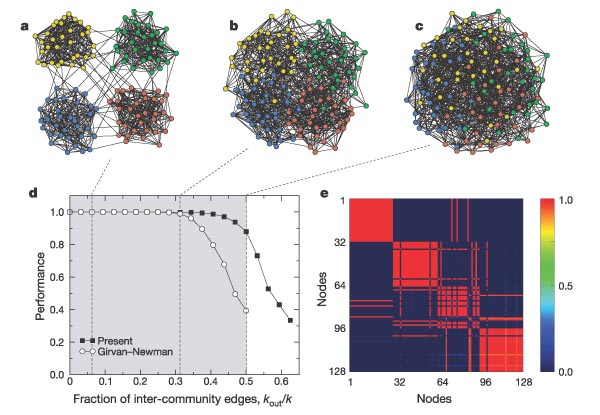
\includegraphics{img/guimera2005_fig1_gm-benchmarks.jpeg}
\caption{Examples of the Girvan-Newman benchmark. From left to right,
the parameter \(z_{out}\) increases (and \(z_{in}\) decreases), and the
community structure becomes less apparent. In (a) \(z_{in}=15\); in (b)
\(z_{in}=11\); and in (c) \(z_{in} = z_{out} = 8\) and the four clusters
are not visually apparent. Image from
\autocite{guimera_functional_2005}.}\label{fig:gn_benchmarks}
\end{figure}

The weakness of the GN benchmarks and the planted \(\ell\)-partition
model in general lies in assumptions that all communities have the same
size and all nodes have the same degree on average. Real-world networks
tend to exhibit skewed, power-law-like distributions for cluster size
and node degree. Lancichinetti et al. have taken steps to address these
issues with their LFR benchmark, which is generally seen as an
improvement over the GN benchmark
\autocites{lancichinetti_benchmark_2008}{fortunato_community_2010}. When
an LFR network is generated, both the degree and cluster size are
assumed to have power law distributions, with exponents \(\gamma\) and
\(\beta\), respectively. The mixing parameter \(\mu\) specifies, for
each node, the fraction of its links that go outside its community. A
graph of \(N\) vertices is generated using a configuration model which
assigns links given the proper degree sequence; the graph is then
rewired with an iterative algorithm until it can be assigned a community
structure with the proper parameters.

\subsection{Evaluation on real-world
networks}\label{evaluation-on-real-world-networks}

A second approach to evaluate community detection methods is to use some
real-world network data and compare the results of the method against
known metadata attributes, which are treated as ground-truth community
structure. The most famous of these networks is the Zachary karate club
dataset \autocite{zachary_information_1977}, which is a network
representation of the social interactions between 34 members of a
university karate club. A conflict between the club president and the
instructor resulted in the formation of two groups of members who had
allegiance to one leader or the other. Community detection methods can
be judged according to how well they are able to infer this group
division from the network structure alone. This network has become so
widely used as a benchmark in network science that researchers who are
first to use it as an example at a conference are awarded a trophy and
inducted into the prestigious ``Zachary Karate Club Club.''\footnote{See
  \url{http://networkkarate.tumblr.com/}} Several other networks have
also emerged as standard benchmarks: Lusseau's network of interaction
between 62 bottlenose dolphins in New Zealand's Doubtful Sound is
compared against a biological classification
\autocite{lusseau_emergent_2003}; and a network in which nodes represent
college football teams and edges represent games played between them is
compared against the known conference divisions of the teams
\autocite{girvan_community_2002}.

The assumption that known metadata can be equated with community
structure has recently begun to be called into question, amid several
findings that most community detection algorithms tend to do a fairly
poor job of recovering these classifications on many large networks
\autocites{yang_defining_2015}{hric_community_2014}. This may represent
something of a crisis for the field.

A very recent paper by Peel et al. breaks down these issues
\autocite{peel_ground_2017}, providing a very interesting and
provocative perspective. While it has been assumed that a method's
failure to recover the metadata associated with the network means that
the method has performed poorly, the authors point out that there are
actually three alternative interpretations: (i) that the metadata do not
actually correspond with network structure, (ii) that the metadata
correspond to a different aspect of the network structure than that
revealed by the community detection method, or (iii) that the network
actually has no detectable community structure. The authors propose a No
Free Lunch theorem for community detection, claiming that no one method
can outperform any other on all cases, implying that methods that have
an advantage for a certain set of cases will have decreased performance
in other cases. They stress that this does not imply that community
detection is a useless endeavor, but they do contend that it is
impossible to find one optimal method, and that efforts should instead
be put into understanding the problem space of different community
detection tasks, so that different algorithms can be developed for each
one. The recent review paper by Schaub et al.
\autocite{schaub_many_2017} is one example of this kind of effort,
classifying and distinguishing the different perspectives on community
detection.

The authors of this study introduce two interesting new statistical
methods to address cases (i) and (ii) in the paragraph above. The first
identifies the extent to which the metadata relates to the network
structure by comparing the entropies of two probabilistic models: one
representing the metadata partitions, and the other a null model with
random permutations of the metadata (this null model preserves network
structure and relative frequencies of metadata values but removes the
correlation between the two). The second statistical method is meant to
shed light on the relatedness between the structural aspects of the
metadata versus the structural aspects that a community detection
algorithm identifies. It does this by imposing a constraint on the
community detection algorithm that fixes some portion of the community
structure produced based on the metadata partitions. By varying this
constraint, one can explore (visually, using a graph) how the imposition
of the metadata affects the likelihood of the community detection
method. Both of these methods are general enough to work with any sort
of probabilistic generative network model; the authors implement them
using stochastic blockmodels (see previous section on community
detection methods), calling the first method the blockmodel entropy
significance test (BESTest), and the second one the neoSBM.

\TODO{2002 girvan and newman paper recognized the idea that metadata might not always be related to network structure. see my note in zotero}

\TODO{Maybe think some more about implications of how community detection is an ill posed problem, and the No Free Lunch theorem}

\subsection{Results of comparative analyses of
algorithms}\label{results-of-comparative-analyses-of-algorithms}

A 2009 paper by Lancichinetti and Fortunato
\autocite{lancichinetti_community_2009} has gained some acceptance in
the network science community as a comparative analysis of the
performance of some of the most popular community detection algorithm.
The 12 algorithms studied included most of those previously discussed
(see section ``\protect\hyperlink{community-detection-methods}{Community
detection methods}''), including the original Girvan-Newman algorithm,
several greedy and more exhaustive modularity-optimizing algorithms, an
Expectation-Maximization Bayesian model-fitting approach similar to
stochastic block models, a spectral algorithm, the Markov cluster
algorithm popular in bioinformatics, and the flow-compression-based
Infomap algorithm of Rosvall and Bergstrom, among several others. They
also included one algorithm that can find overlapping partitions, called
Cfinder.

The algorithms were tested on random graphs generated using the LFR
method (see section
``\protect\hyperlink{synthetic-benchmark-networks}{Synthetic benchmark
networks}''; these benchmark graphs are more rigorous than the
Girvan-Newman benchmarks that came before. The results were compared
using their variant of normalized mutual information (see section
``\protect\hyperlink{comparison-measures}{Comparison measures}'').
Briefly, the results were as follows: The original Girvan-Newman
algorithm suffered from too many performance issues to be considered,
failing to finish on most networks (the authors included this method
mostly for historical reasons; the other methods are more modern and
improved). The modularity-based methods tended to suffer from that
approaches resolution limit (see section
``\protect\hyperlink{the-clustering-perspective}{The clustering
perspective}''), failing to detect smaller planted communities on larger
graphs. The authors concluded that Infomap was overall the best
performing algorithm, with good performance on different sized graphs,
and also directed and weighted graphs. It was also one of the fastest
methods, along with the Louvain method---the authors were able to test
these two on larger graphs (up to 100,000 nodes), and only Infomap
maintained good performance. The study did not study hierarchical
partitions, or the overlapping or higher-order versions of Infomap.

The authors also test the methods on random graphs. An algorithm taking
as input a random graph, in which every pair of nodes having an equal
probability of being linked, should not find a community structure, but
this is not always the case (see section
\protect\hyperlink{confidence-in-communities}{``Confidence in
communities''}). Methods based on modularity fall short here, finding
some communities in random graphs. Infomap tends to perform better,
finding a single module comprising all nodes. However, Infomap still
does find some community structure when the average degree of the nodes
is low---i.e., the graph is sparse. This could pose a problem, as many
real-world graphs are sparse.

\TODO{emmons/borner paper. see "Comparison of Clustering Algorithms" section: they use benchmarks with a large community size. this works in the favor of Louvain, which has modularity's resolution limit. (they take the bottom level of Infomap's hierarchy)}

\TODO{remark on how LFR benchmarks are based on SBMs, so they would be expected to score best. can find this in fortunato and hric 2016 (and also i think in schaub 2017)}

\subsection{Visualization}\label{visualization}
